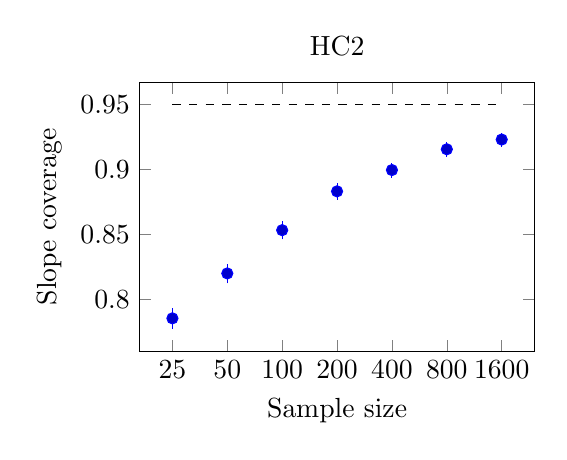
\begin{tikzpicture}
\begin{axis}[width=6.6cm,height=5cm,xlabel={Sample size},ylabel={Slope coverage},title={HC2},xtick={0,1,2,3,4,5,6},xticklabels={{25},{50},{100},{200},{400},{800},{1600}}]
% Interval meaning: Wilson 95% interval for coverage over 10000 trials
\addplot+[no marks,forget plot] coordinates {(0,0.7772446798874184) (0,0.7933361338425993)};
\addplot+[no marks,forget plot] coordinates {(1,0.8123476279170886) (1,0.8274066131256782)};
\addplot+[no marks,forget plot] coordinates {(2,0.846229855766208) (2,0.8600988109850718)};
\addplot+[no marks,forget plot] coordinates {(3,0.8767572927270054) (3,0.8893484109217079)};
\addplot+[no marks,forget plot] coordinates {(4,0.8935553559860696) (4,0.9053377525160855)};
\addplot+[no marks,forget plot] coordinates {(5,0.9099906788405526) (5,0.9208901417137408)};
\addplot+[no marks,forget plot] coordinates {(6,0.9177140205011988) (6,0.9281610400775347)};
\addplot+[only marks,forget plot] coordinates {(0,0.7854) (1,0.82) (2,0.8533) (3,0.8832) (4,0.8996) (5,0.9156) (6,0.9231)};
\addplot[black,dashed,no marks,forget plot] coordinates {(0,0.95) (6,0.95)};
\end{axis}
\end{tikzpicture}
